\documentclass[journal=jcisd8,manuscript=article]{achemso}
\usepackage{graphicx}
\usepackage{xr-hyper}
\usepackage{hyperref}
\usepackage{xcolor}
\usepackage{verbatim}
\usepackage[subrefformat=parens]{subcaption}
\usepackage[finalizecache,cachedir=.]{minted}
\usepackage[version=3]{mhchem} % Formula subscripts using \ce{}

\renewcommand{\thetable}{S\arabic{table}}  
\renewcommand{\thefigure}{S\arabic{figure}}

\author{Paul G. Francoeur}
\author{David R. Koes}
\email{dkoes@pitt.edu}
\affiliation[Pitt]{Department of Computational and Systems Biology, University of Pittsburgh, Pittsburgh, PA 15260}

\title{Supporting Information:\\SolTranNet -- A ML tool for fast aqueous solubility prediction.}
\begin{document}
\begin{table}
    %\centering
    \begin{tabular}{|c|c|c|c|c|c|c|}
        \hline
         Model & Parameters & CCV $R^2$ & Fold0 $R^2$ & Fold1 $R^2$ & Fold2 $R^2$ & Ind $R^2$ \\
         \hline
         MAT & 42,049,537 & 0.532 & 0.751 & 0.332 & 0.715 & 0.375  \\
         \hline
         0 & 21,061,633 & 0.670 & 0.778 & 0.520 & 0.727 & 0.4718 \\
         1 & 502,529 & 0.662 & 0.769 & 0.465 & 0.733 & 0.4576 \\
         2 & 336,385 & 0.693 & 0.764 & 0.563 & 0.706 & 0.4890 \\
         3 & 336,385 & 0.672 & 0.764 & 0.539 & 0.685 & 0.4461 \\
         4 & 22,657 & \textbf{0.724} & 0.780 & \textbf{0.626} & 0.716 & 0.4831 \\
         5 & 11,905 & \textbf{0.723} & \textbf{0.793} & 0.595 & 0.744 & 0.4628 \\
         6 & 11,905 & 0.713 & 0.786 & 0.582 & \textbf{0.756} & 0.4517 \\
         \emph{7} & \emph{3,393} & \emph{0.6764} & \emph{0.7914} & \emph{0.5243} & \emph{0.7424} & \emph{\textbf{0.5528}}\\
         8 & 2,609 & 0.695 & 0.779 & 0.545 & 0.737  & 0.4589\\
         9 & 2,609 & 0.677 & 0.767 & 0.552 & 0.720  & 0.4678\\
         \hline
         Elastic & 1,463 & 0.414 & 0.441 & 0.394 & 0.408  & 0.377\\
         Lasso & 1,077 & 0.395 & 0.409 & 0.378 & 0.392  & 0.351\\
         PLS & 2,048 & 0.228 & 0.212 & 0.333 & 0.0747  & 0.676\\
         Ridge & 2,048 & 0.319 & 0.289 & 0.354 & 0.291 & 0.261 \\
         \hline
    \end{tabular}
    \caption{SolTranNet hyperparameter search correlations. There is a general trend of models with fewer parameters performing better. Additionally, all models significantly outperform linear ML approaches. The model in italics is the final model selection.}
    \label{tab:solsearchr2}
\end{table}


\begin{table}
    %\centering
    \begin{tabular}{|c|c|}
        \hline
         Index & Description \\
         \hline
         0-11 & Atom Identity as one-hot (B,N,C,O,F,P,S,Cl,Br,I,Dummy,Other) \\
         12-17 & Number of heavy atom neighbors as one-hot of 0-5 \\
         18-22 & Number H atoms as one-hot of 0-4 \\
         23 & Formal Charge \\
         24 & In a Ring \\
         25 & Armoatic \\
         \hline
    \end{tabular}
    \caption{Featurization used to embed atoms in SolTranNet. This is the same schema as in the original MAT implementation. }
    \label{tab:atomembed}
\end{table}


\begin{figure}[tb]
    \centering
    \begin{subfigure}[t]{0.48\textwidth}
        \centering
        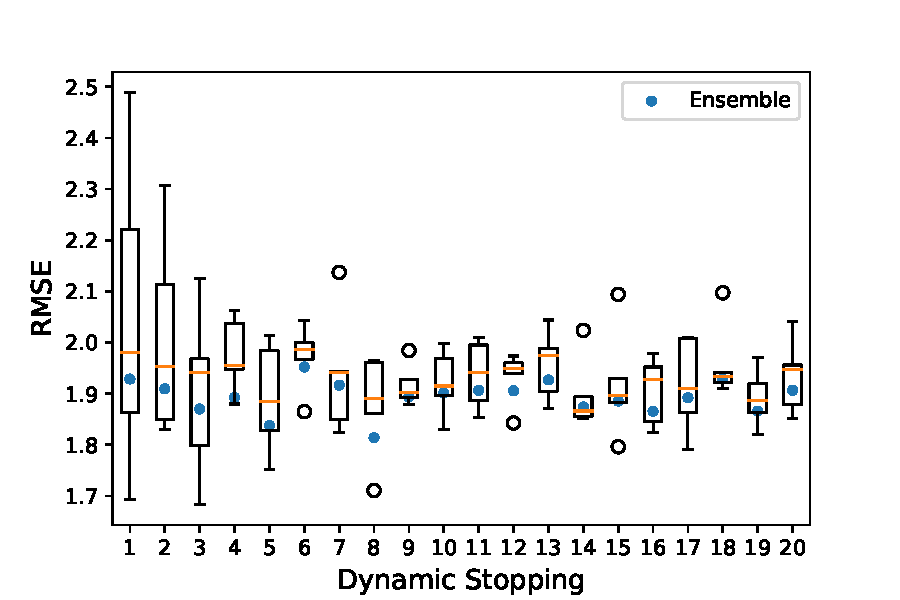
\includegraphics[width=\linewidth]{figures/final_model_ind_dyn_RMSE.pdf}
    \end{subfigure}%
    \hfill
    \begin{subfigure}[t]{0.48\textwidth}
        \centering
        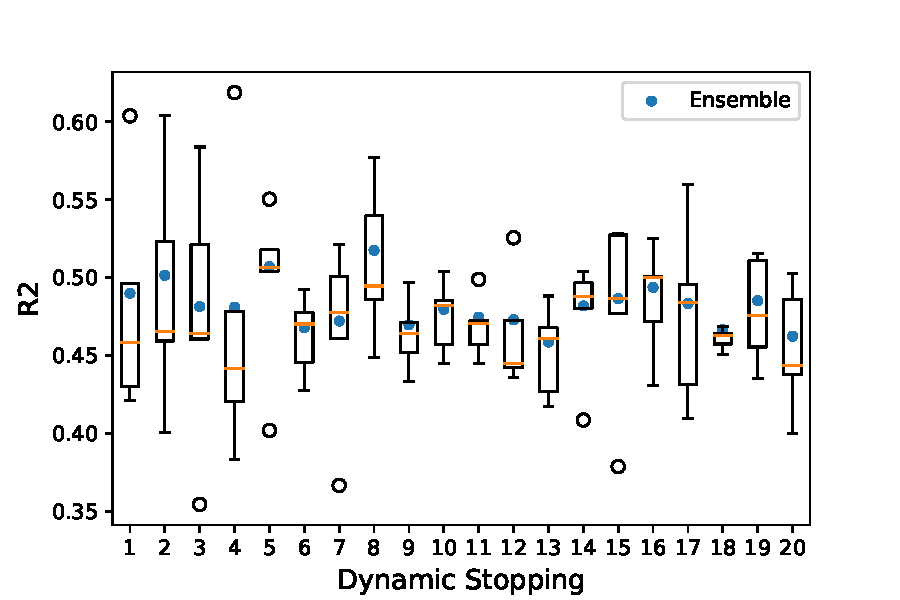
\includegraphics[width=\linewidth]{figures/final_model_ind_dyn_R2.pdf}
    \end{subfigure}
    \caption{Boxplots of the performance of SolTranNet models on our independet test set using various dynamic stopping criteria. The Dynamic Stopping is the number of epochs that the model can fail to improve its fit to the training set before training is stopped. The boxplot is of 5 different seeds, with the ensemble performance shown with the blue dot. Interestingly, the ensemble outperforms the mean performance of the 5 models, but fails to be better than the best performing seed in all cases.}
    \label{fig:dynsweep}
\end{figure}

\begin{figure}[tb]
    \centering
    \begin{subfigure}[t]{0.48\textwidth}
        \centering
        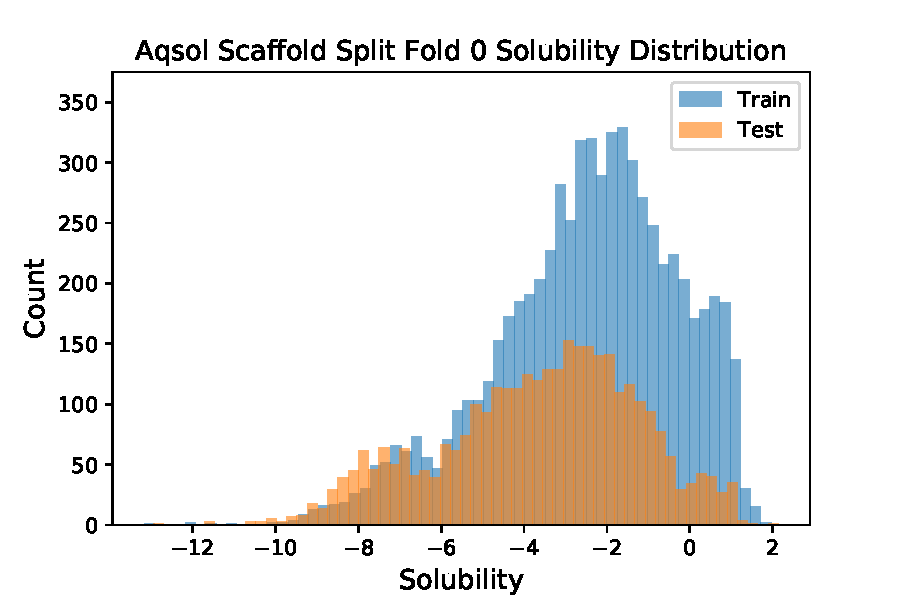
\includegraphics[width=\linewidth]{figures/aqsol_scaf0_soldist.pdf}
    \end{subfigure}%
    \hfill
    \begin{subfigure}[t]{0.48\textwidth}
        \centering
        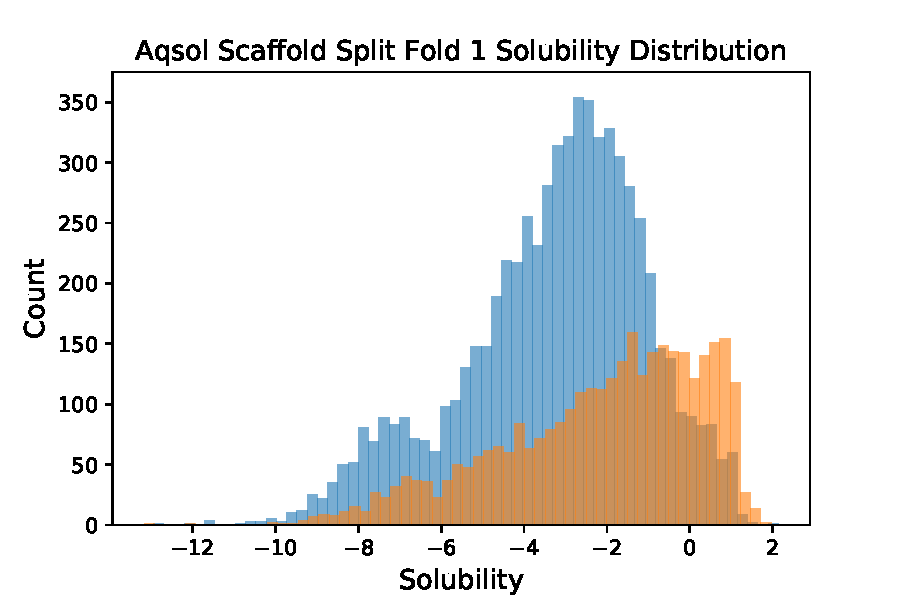
\includegraphics[width=\linewidth]{figures/aqsol_scaf1_soldist.pdf}
    \end{subfigure}
    
    \begin{subfigure}[t]{0.48\textwidth}
        \centering
        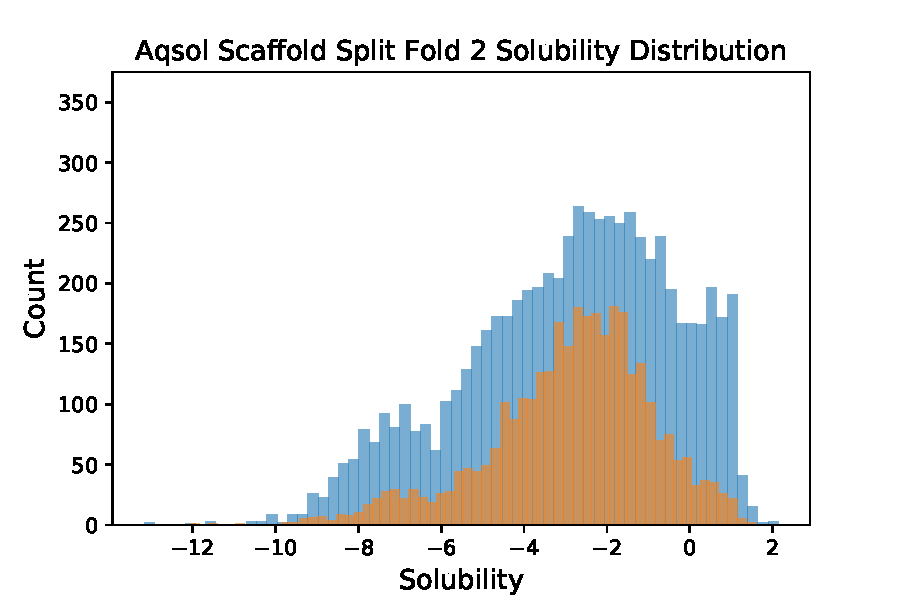
\includegraphics[width=\linewidth]{figures/aqsol_scaf2_soldist.pdf}
    \end{subfigure}
    
    
    \begin{subfigure}[t]{0.48\textwidth}
        \centering
        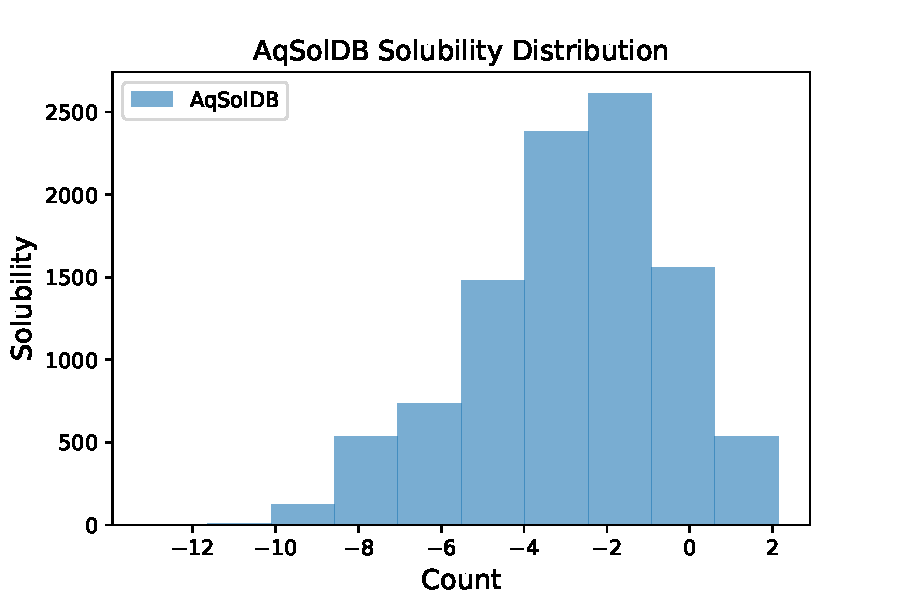
\includegraphics[width=\linewidth]{figures/AqSolDB_solhist.pdf}
    \end{subfigure}%
    \hfill
    \begin{subfigure}[t]{0.48\textwidth}
        \centering
        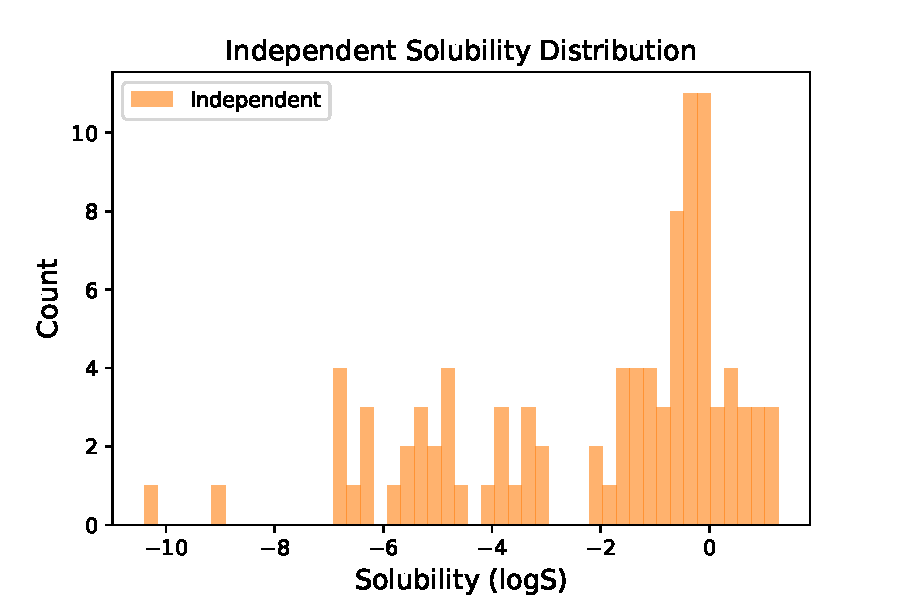
\includegraphics[width=\linewidth]{figures/Independent_solhist.pdf}
    \end{subfigure}
    \caption{Distributions of our various training set data. Each bin }
    \label{fig:solhists}
\end{figure}



\end{document}